%-------------------------------------------------------------------------------
%	CAPITOLO 32
%-------------------------------------------------------------------------------

\chapter{Ho trovato un tesoro}

Eravamo nel periodo, dopo le bande dei ladri. La maggioranza dei ladri erano ancora in galera, ed il popolo fantasticava sulle dicerie che il tale aveva confessato ad un amico di galera di aver seppellito una pentola e marenghi d'oro rubati in qua in là.\\
\indent I luoghi indicati erano la \index[Luoghi]{Chiesa della Madonna del Bosco}chiesa della Madonna dei Boschi, il \index[Luoghi]{Pilastrino della Madonna}Pilastrino della Madonna, ecc... Spesso si vedevano in luogo scavi e tentativi di recupero della gran pentola col tesoro e le fantasie correvano.\\
\indent Una notte il buon \index[Personaggi]{N\:.\:.\:.}N\:.\:.\:. era a letto con la sua \index[Personaggi]{T\:.\:.\:.}T\:.\:.\:. quando lo sveglia un gran pugno tra capo e collo e la voce irata della donna: <<Guarda che cos'hai fatto...>>\\
\indent \index[Personaggi]{N\:.\:.\:.}N\:.\:.\:. ancora mezzo addormentato e in istato di subcoscenza rispose: <<Sta bona la mi \index[Personaggi]{T\:.\:.\:.}T\:.\:.\:. aiò truvé un tesor in te pre dla Madona, e par fei e segn par trovél, aiò caghé in sò.\footnote{<<Sta buona la mia T\:.\:.\:. ho trovato un tesoro nel prato della Madonna e per fargli un segno e trovarlo vi ho cagato sopra>>}>>\\
\indent \index[Personaggi]{T\:.\:.\:.}T\:.\:.\:. : <<E tesor l'è che tamé caghé  in su na gamba e in te let.\footnote{"Il tesoro è che mi hai cagato su di una gamba e nel letto.>>}>>\\
\indent Il resto del risveglio fu molto più reale... perché dovettero alzarsi e preparare il bucato...


\begin{figure}[hbt]%
	\vspace{-1cm}
    \centering
    \subfloat[Il santuario della Madonna dei Boschi]{{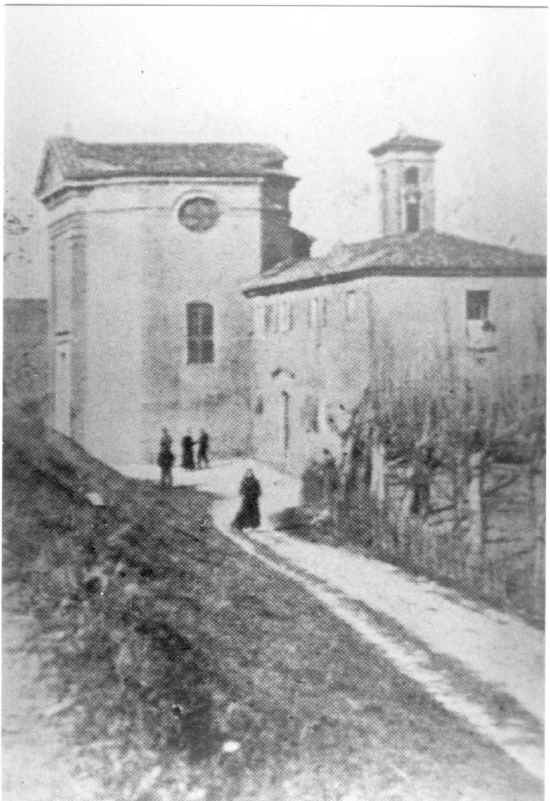
\includegraphics[height=8cm]{santuario}}}%
    \subfloat[Il Pilastrino della Madonna]{{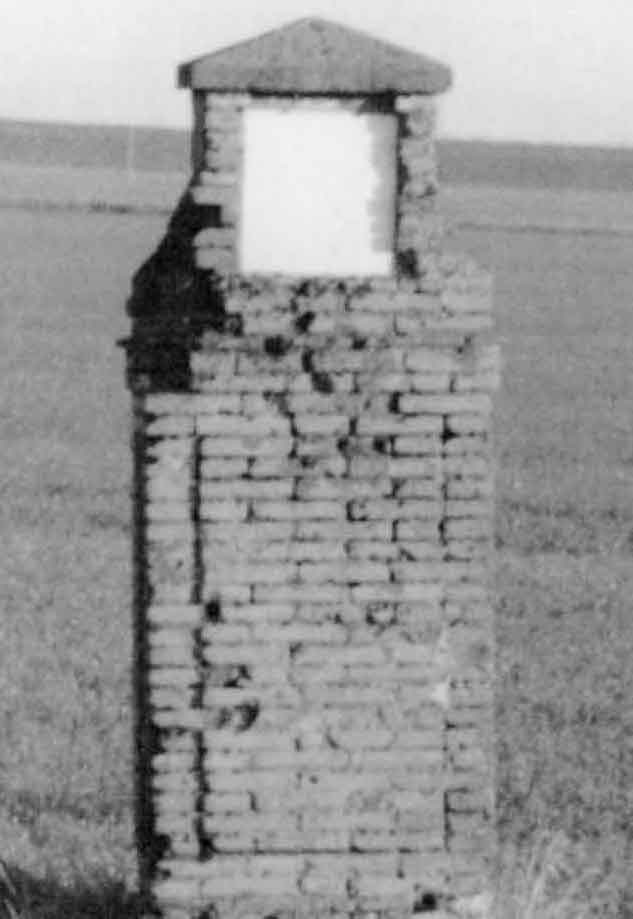
\includegraphics[height=8cm]{pilastrino} }}%
	\vspace{-0.2cm}
\end{figure}